\newcommand{\posterAccelerator}[1]{

\setlength{\frameWidth}{#1}
\setlength{\unitlength}{0.02\frameWidth}
\psset{unit=\unitlength}

\rput(25,14){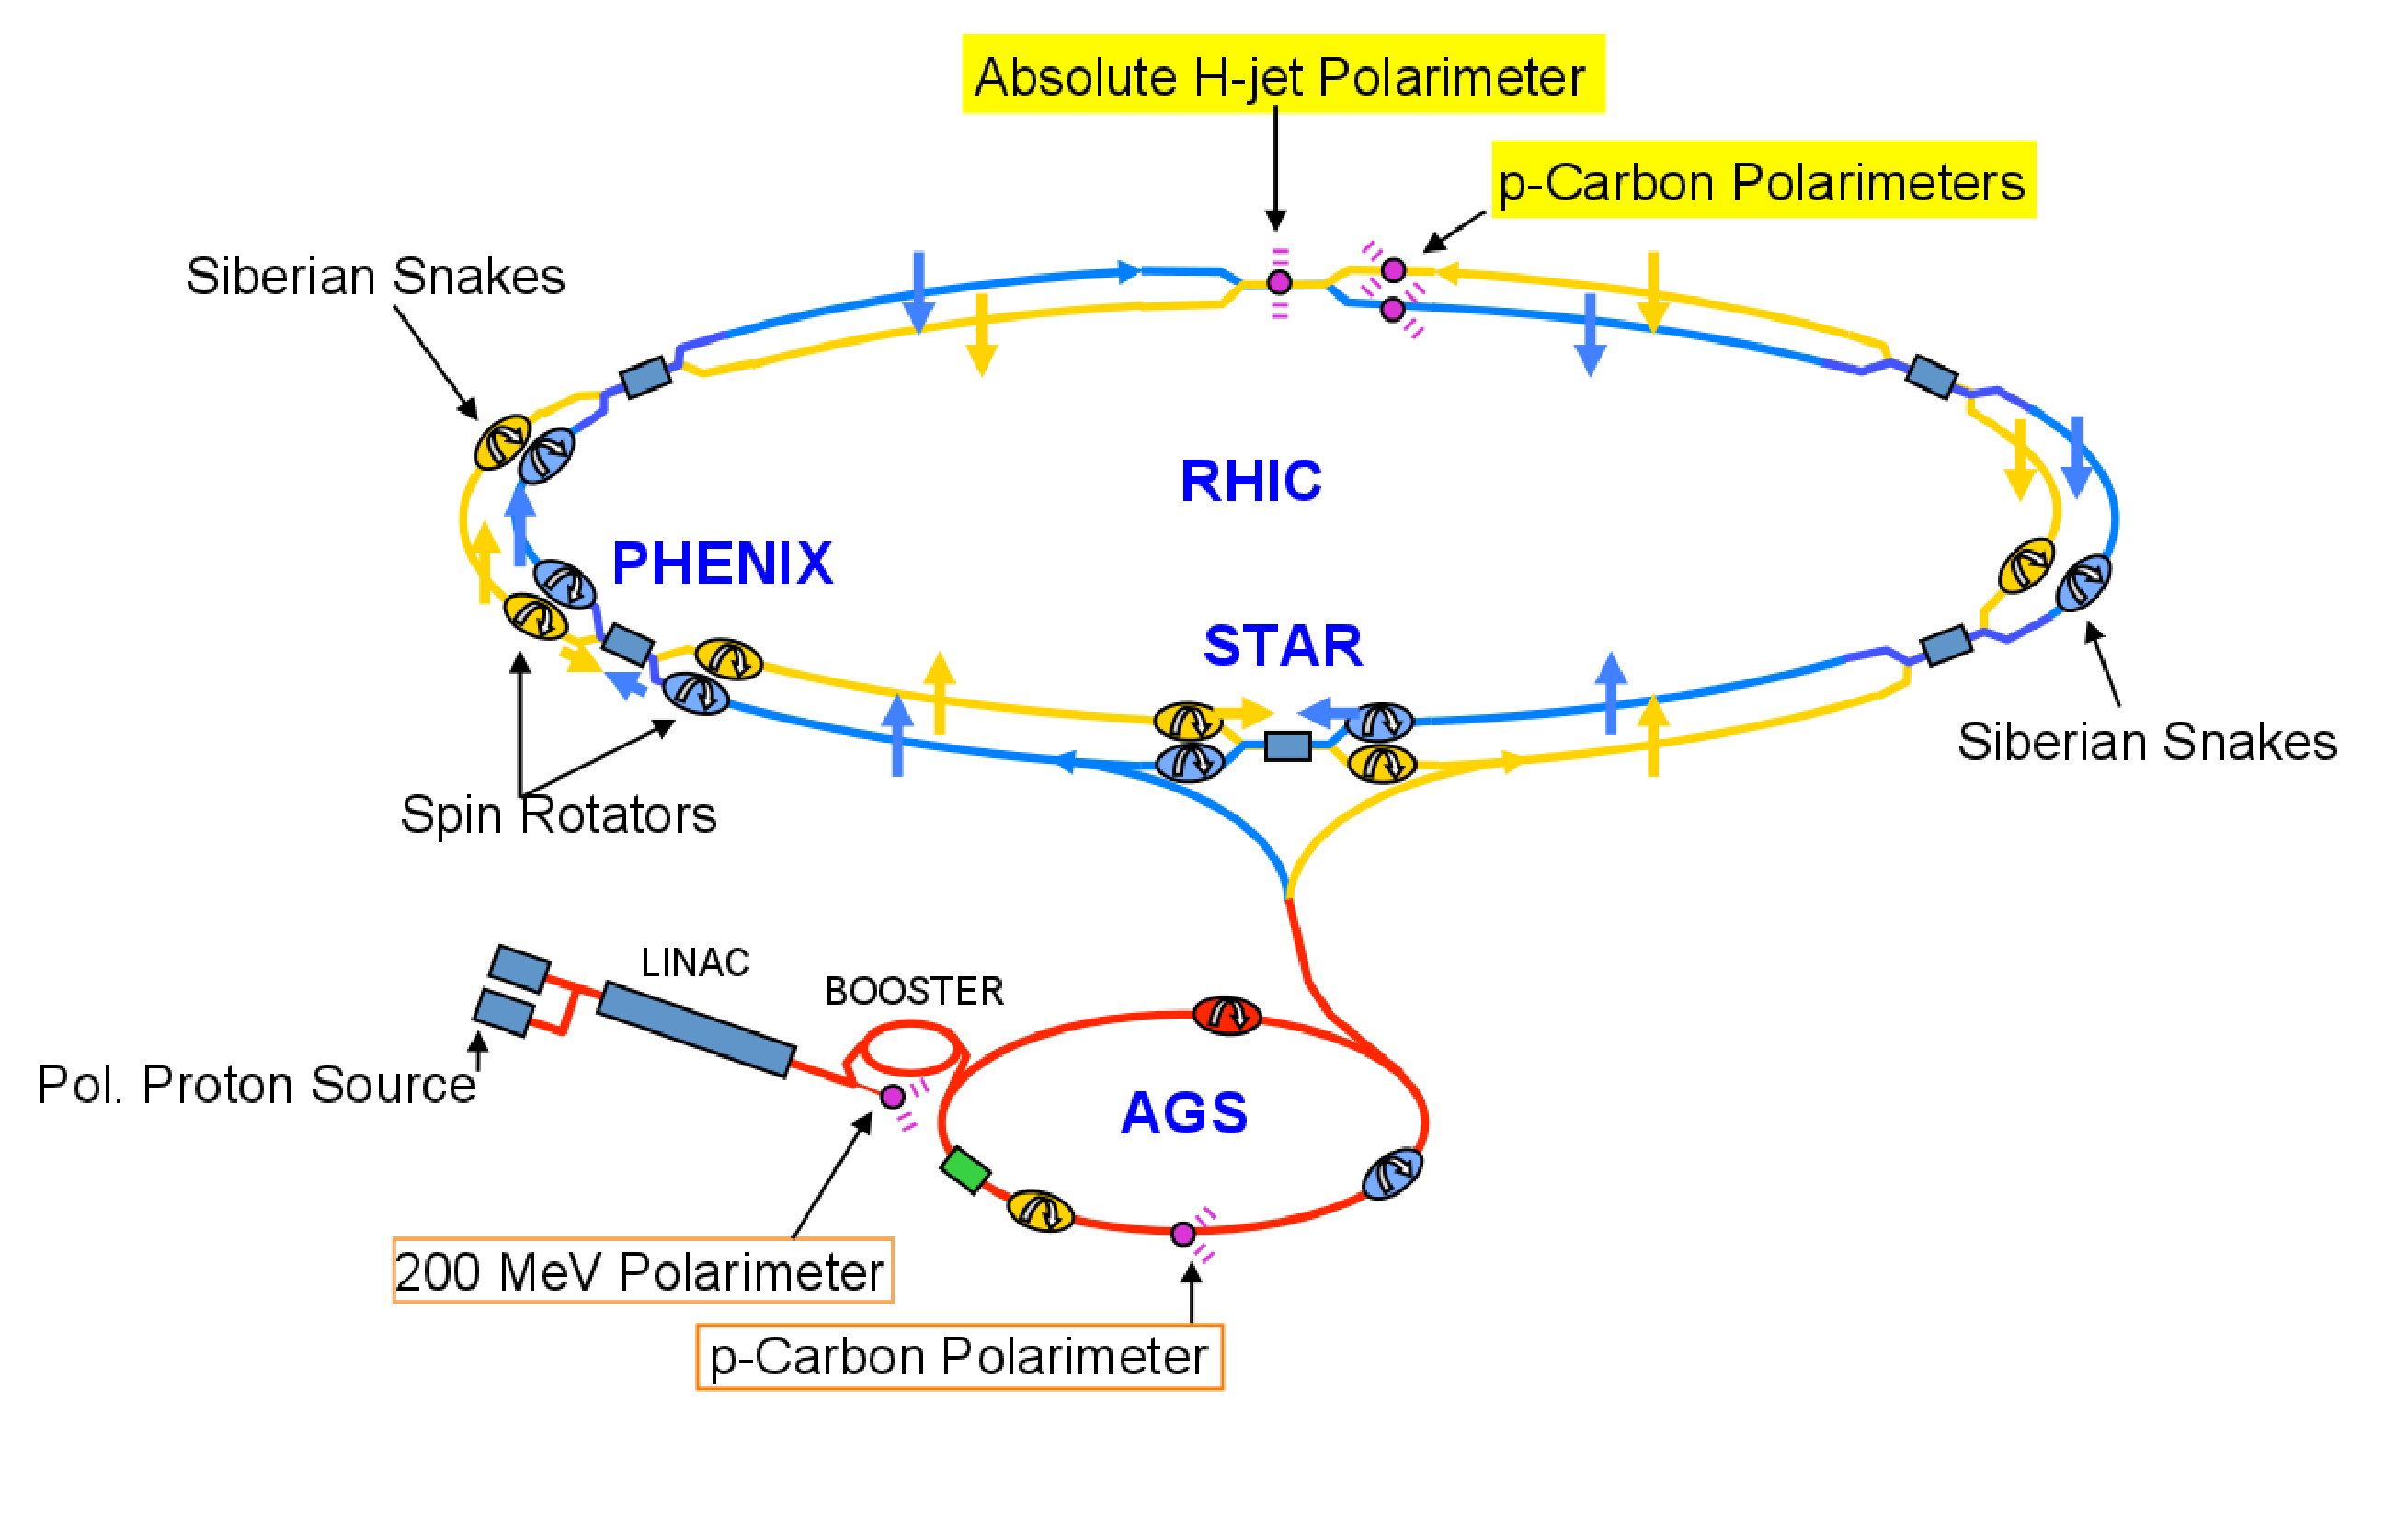
\includegraphics[width=50\unitlength]{graphics/rhic_ags}}

\rput[lt](31,13) {%
\psframebox[framearc=.1,fillcolor=blue!10,linecolor=blue!10,linewidth=.8mm,fillstyle=solid]{%
\parbox{17\unitlength}{%
\begin{minipage}{17\unitlength}

\raggedright

\begin{list}{\labelitemi}{\setlength{\itemsep}{-3mm}
                          \setlength{\topsep}{0mm}}

   %\item 120 bunches ($\sim 110$~ns) across the ring
   \item RHIC rings filled with $\sim 120 \times 10^{11}$ protons
   \item Beams cross at rate of $\sim 9$~MHz
   \item Collisions with all spin combinations available\\
   {\boldmath $\uparrow\uparrow$, $\uparrow\downarrow$, $\downarrow\uparrow$, $\downarrow\downarrow$}

\end{list}

\end{minipage}
} } }

%\rput{0}{\psgrid[gridlabels=0.7,subgriddiv=0, griddots=3](1,-1)(0,0)(\myPsPictureWidthLocal,\myPsPictureHeightLocal)}

}

\setlength{\unitlength}{10mm}
\psset{unit=\unitlength}
